\chapter{Complete Project Ecosystem}
\label{ch:complete-project-ecosystem}

\section{Problem Definition and Threat Landscape}
\label{sec:problem}

Modern digital forensics and cyber threat intelligence (CTI) face severe operational fragmentation when investigating illicit actors across multi-jurisdiction, decentralized online ecosystems \cite{liao2016acing, soska2015measuring}. Sophisticated threat actors routinely fragment their operational identities across independent forums, darknet marketplaces, escrow exchanges, and portfolio networks to prevent cross-platform correlation. Traditional entity resolution (ER) systems \cite{fellegi1969theory, getoor2012entity} are typically engineered for centralized enterprise databases with uniform schemas, high attribute completeness, and cooperative data owners. In contrast, adversarial cyber threat intelligence requires resolving identities from uncooperative, heterogeneous, and ephemeral platforms characterized by rapid contract drift, deliberate alias mutation, and temporal uncertainty \cite{narayanan2008robust, elmagarmid2007duplicate}.

Furthermore, investigating real-world criminal infrastructure presents significant legal, ethical, and privacy barriers: harvesting live darknet communications risks processing sensitive real-world Personal Identifiable Information (PII) without consent \cite{dwork2006differential}. To overcome this research barrier, synthetic population modeling has emerged as a vital methodology, enabling repeatable evaluation without privacy violations \cite{nowok2016synthpop}. The overarching challenge addressed by the \textit{Wolverine} ecosystem is constructing an end-to-end, deterministic intelligence architecture that can ingest multi-protocol synthetic data, resolve cross-platform identities without ground-truth leakage, project traversable relationship graphs with bounded compute, and maintain an immutable cryptographic audit ledger.

\section{Formal Engineering and Research Questions}
\label{sec:research_questions}

To guide the design and empirical qualification of the system, we formalize three central research and engineering questions:

\begin{itemize}
    \item \textbf{EQ-1 (Multi-Source Heuristic Precision):} Can a composite similarity ensemble combining prefix blocking, Jaro-Winkler string metrics \cite{jaro1989advances, winkler1990string}, and linear temporal proximity achieve high precision ($\ge 90\%$) across heterogeneous schema paradigms without oracle ground-truth access?
    \item \textbf{EQ-2 (Bounded In-Memory Topological Exploration):} How effectively does an in-memory Bounded Breadth-First Search (BFS) ($d \le 4, N \le 500$) guarantee deterministic query bounds compared to unbounded relational recursions or heavy graph database engines \cite{newman2003structure, cormen2009introduction}?
    \item \textbf{EQ-3 (Cryptographic Auditability under Simulated Transport):} Can an independent cryptographic trust layer (WolverineDB) enforce verifiable append-only state integrity and Byzantine Fault Tolerant (BFT) consensus \cite{castro2002practical, merkle1987digital} when evaluated within an in-process simulated transport environment?
\end{itemize}

\section{Ecosystem Architecture and Repository Decomposition}
\label{sec:design}

The Wolverine ecosystem is structurally decomposed into four distinct, loosely-coupled repositories and microservices:

\begin{itemize}
    \item \textbf{\texttt{wolverine-sih}}: The central intelligence monorepo. It encompasses the multi-protocol collection adapters, canonical normalization parsers, Redis Streams event dispatcher, Jaro-Winkler entity resolution engine, in-memory graph projector, sanitized RAG assistant, and the React-based Analyst UI.
    \item \textbf{\texttt{wolverine-db}}: A standalone cryptographic state middleware library (v1.3.0). It enforces tamper-evident change auditing via SHA-256 hash chains, RFC~6962 Merkle trees, RFC~8785 JSON canonicalization, and 4-of-5 BFT validator consensus.
    \item \textbf{\texttt{Vzeya}}: A cinematic Next.js 15 / React 19 presentation frontend. It provides interactive 3D WebGL particle simulations alongside a lightweight CSS \texttt{repeating-linear-gradient} CRT overlay, serving as a tactical demonstration interface over static mock data.
    \item \textbf{\texttt{generator}}: A 12-phase deterministic synthetic data generator. It populates five heterogeneous web platforms (Atlas Market, Briar Bazaar, Cinder Exchange, Drift Forum, and Ember Commons) with 50,000 synthetic personas while isolating ground-truth mappings in a logically air-gapped PostgreSQL vault (\texttt{postgres-truth}).
\end{itemize}

\begin{figure}[htpb]
\centering
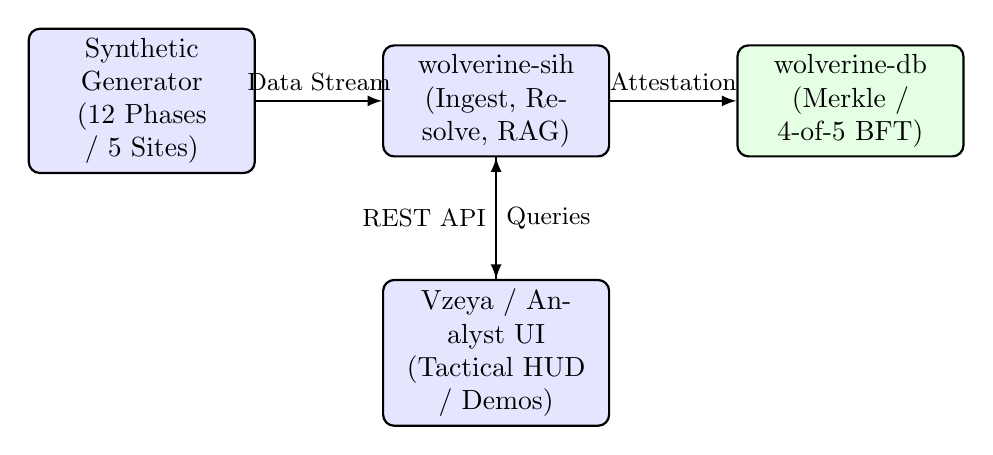
\begin{tikzpicture}[node distance=2.2cm, auto, thick, >=stealth]
  \tikzstyle{block} = [rectangle, draw, fill=blue!10, text width=7.5em, text centered, rounded corners, minimum height=3.5em]
  \tikzstyle{dbnode} = [rectangle, draw, fill=green!10, text width=7.5em, text centered, rounded corners, minimum height=3.5em]
  \tikzstyle{line} = [draw, -latex]

  \node [block] (gen) {Synthetic Generator\\(12 Phases / 5 Sites)};
  \node [block, right of=gen, node distance=4.5cm] (sih) {wolverine-sih\\(Ingest, Resolve, RAG)};
  \node [dbnode, right of=sih, node distance=4.5cm] (db) {wolverine-db\\(Merkle / 4-of-5 BFT)};
  \node [block, below of=sih, node distance=3.2cm] (vzeya) {Vzeya / Analyst UI\\(Tactical HUD / Demos)};

  \path [line] (gen) -- node[above] {\small Data Stream} (sih);
  \path [line] (sih) -- node[above] {\small Attestation} (db);
  \path [line] (sih) -- node[left] {\small REST API} (vzeya);
  \path [line] (vzeya) -- node[right] {\small Queries} (sih);
\end{tikzpicture}
\caption{Wolverine Ecosystem Macro-Architecture and Inter-Repository Topology}
\label{fig:architecture}
\end{figure}

\section{Core Implementation Principles}
\label{sec:implementation}

The software implementation enforces strict technical and mathematical boundaries derived from source code:

\subsection{Linear Temporal Decay and Dual Thresholds}
Entity resolution relies on historical evidence whose investigative relevance decays over time. The system implements a strict linear 30-day temporal decay model ($S_{temporal} = \max(0, 1 - \frac{\Delta t}{30\text{ days}})$), deliberately avoiding non-linear exponential models to guarantee mathematical predictability across long simulation timelines. Record pairs are classified via a bipartite threshold: an automatic merge threshold of $S \ge 0.92$ and an analyst review threshold of $0.70 \le S < 0.92$.

\subsection{Byzantine Fault Tolerant State Verification}
WolverineDB implements a 4-of-5 BFT consensus engine to validate relational state mutations. Because distributed physical networking is decoupled in the SIH demonstration environment, validator attestations and Quorum Certificates are transmitted synchronously via a simulated \texttt{DirectMemoryNetworkTransport} layer.

\subsection{In-Memory Bounded BFS Graph Projection}
Graph relationships are projected dynamically from canonical records and resolution candidates into in-memory adjacency maps (\texttt{GraphProjector}). Analytical queries execute a bounded BFS constrained strictly to $d \le 4$ and $N \le 500$ records, eliminating recursive database lock contention.

\section{Evidentiary Qualification and Limitations}
\label{sec:limitations}

While the Wolverine prototype demonstrates functional integration across all pipelines, its findings are bounded by specific methodological limitations: (1) data is entirely synthetic, meaning real-world adversarial evasion (e.g., advanced homoglyph obfuscation or temporal jitter) is not fully represented; (2) consensus validation is verified within a single-process memory transport rather than a multi-node WAN; and (3) static baseline metrics ($P=0.9280, R=0.4598$) reflect reference test fixtures rather than dynamic empirical distributions.

\section{Research Significance}
\label{sec:significance}

The Wolverine ecosystem contributes an integrated reference architecture for multi-source threat intelligence. By pairing deterministic heuristic entity resolution with in-memory graph projection and cryptographic state verification, it demonstrates that complex cross-platform attribution pipelines can be evaluated safely, verifiably, and with bounded compute.
